\chapter{Case Study 4: Interactive TV}

\section{Introduction}

An increasing number of interactive applications can be downloaded
onto devices such as mobile phones, PDAs, web-browsers and TV set-top
boxes. The applications involve presenting the user with information,
options, menus and buttons. The user typically enters information
by typing text and choosing amongst alternatives. An event is generated
by the user clicking a button or selecting from a menu. Once an event
is generated an engine that services the interactive application processes
the event, updates its internal state and then produces a new dialog
to present to the user.

The dialogs required by the interactive applications tend to be fairly
simple and are often used in conjunction with other applications such
as being broadcast together with TV video and audio content. The technology
used to construct the interactive application should be accessible
to as broad a spectrum of users as possible, including users whose
primary skill is not in developing interactive software applications.

Technologies used for interactive displays include Java-based technologies
such as the Multimedia Home Platform (MHP)\cite{MHP} , HTML and JavaScript.
These technologies are very platform specific. They include a great
deal of technical detail and are certainly not approachable by a non-specialist.
Furthermore, the general low-level nature of the technologies does
not enforce any standard look-and-feel to interactive applications.
The applications developed for a given client (for example a single
TV company) should have a common look and feel that is difficult to
enforce at such a low-level.

A common way to abstract from technical detail and to enforce a common
look-and-feel for a suite of applications it to develop a \emph{domain-specific
language} (DSL) whose concepts match the expectations and skill-levels
of the intended users. A DSL for interactive applications will include
constructs for expressing textual content, buttons and choices. The
DSL leaves the rendering of the display features and the event generation
to a display engine that enforces a given look-and-feel. The display
engine can be replaced, changing the look-and-feel without changing
the DSL.

In addition to the DSL supporting high-level features for expressing
display content, it must provide some means for describing what the
application \emph{does}. Normally, application processing algorithms
are expressed at a low-level in program-code. If the DSL is designed
with an \emph{execution engine} then the same approach to abstraction
from rendering detail can be applied to abstraction from the operational
detail.

An executable DSL is a language for expressing complete applications
without detailed knowledge of implementation technologies. The xDSL
is a modelling language, instances of which are expressed as data.
An execution engine processes the data and runs the application. The
xDSL engine can be embedded within devices and other software applications
in order to run the models.

This chapter describes the design of an xDSL for interactive applications.
The xDSL has a textual syntax and is implemented in the tool XMF.
XMF is a platform for developing DSL-based applications. It provides
an extensive high-level language called XOCL for developing applications
and XOCL can be extended with new language constructs. The design
of XMF has been based on Common Lisp \cite{Lisp}, Smalltalk, Scheme
\cite{Scheme} and ObjVLisp \cite{objVlisp}. The DSL for interactive
applications described in this chapter can be developed on any platform,
but XMF is ideally suited to the task.

The rest of this chapter is structured as follows: section \ref{sec:Interactive-Application-Architecture}
describes an architecture for interactive applications based on an
xDSL; section \ref{sec:A-DSL-for-Interactive-Applications} describes
the xDSL from the point of view of the application developer, it outlines
the language features in terms of a simple application involving a
quiz; section \ref{sec:Implementation} describes how the xDSL is
implemented on XMF; section \ref{sec:Simulation} shows how the rendering
engine can be simulated and connected to the xDSL engine to simulate
the execution of an interactive application; section \ref{sec:XML-Representation-for}
shows how the application models can be serialized as XML; section
\ref{sec:Conclusion} concludes by reviewing the key features of the
approach and the technology used to develop the xDSL engine.


\section{Interactive Application Architecture\label{sec:Interactive-Application-Architecture}}

%
\begin{figure}
\begin{center}
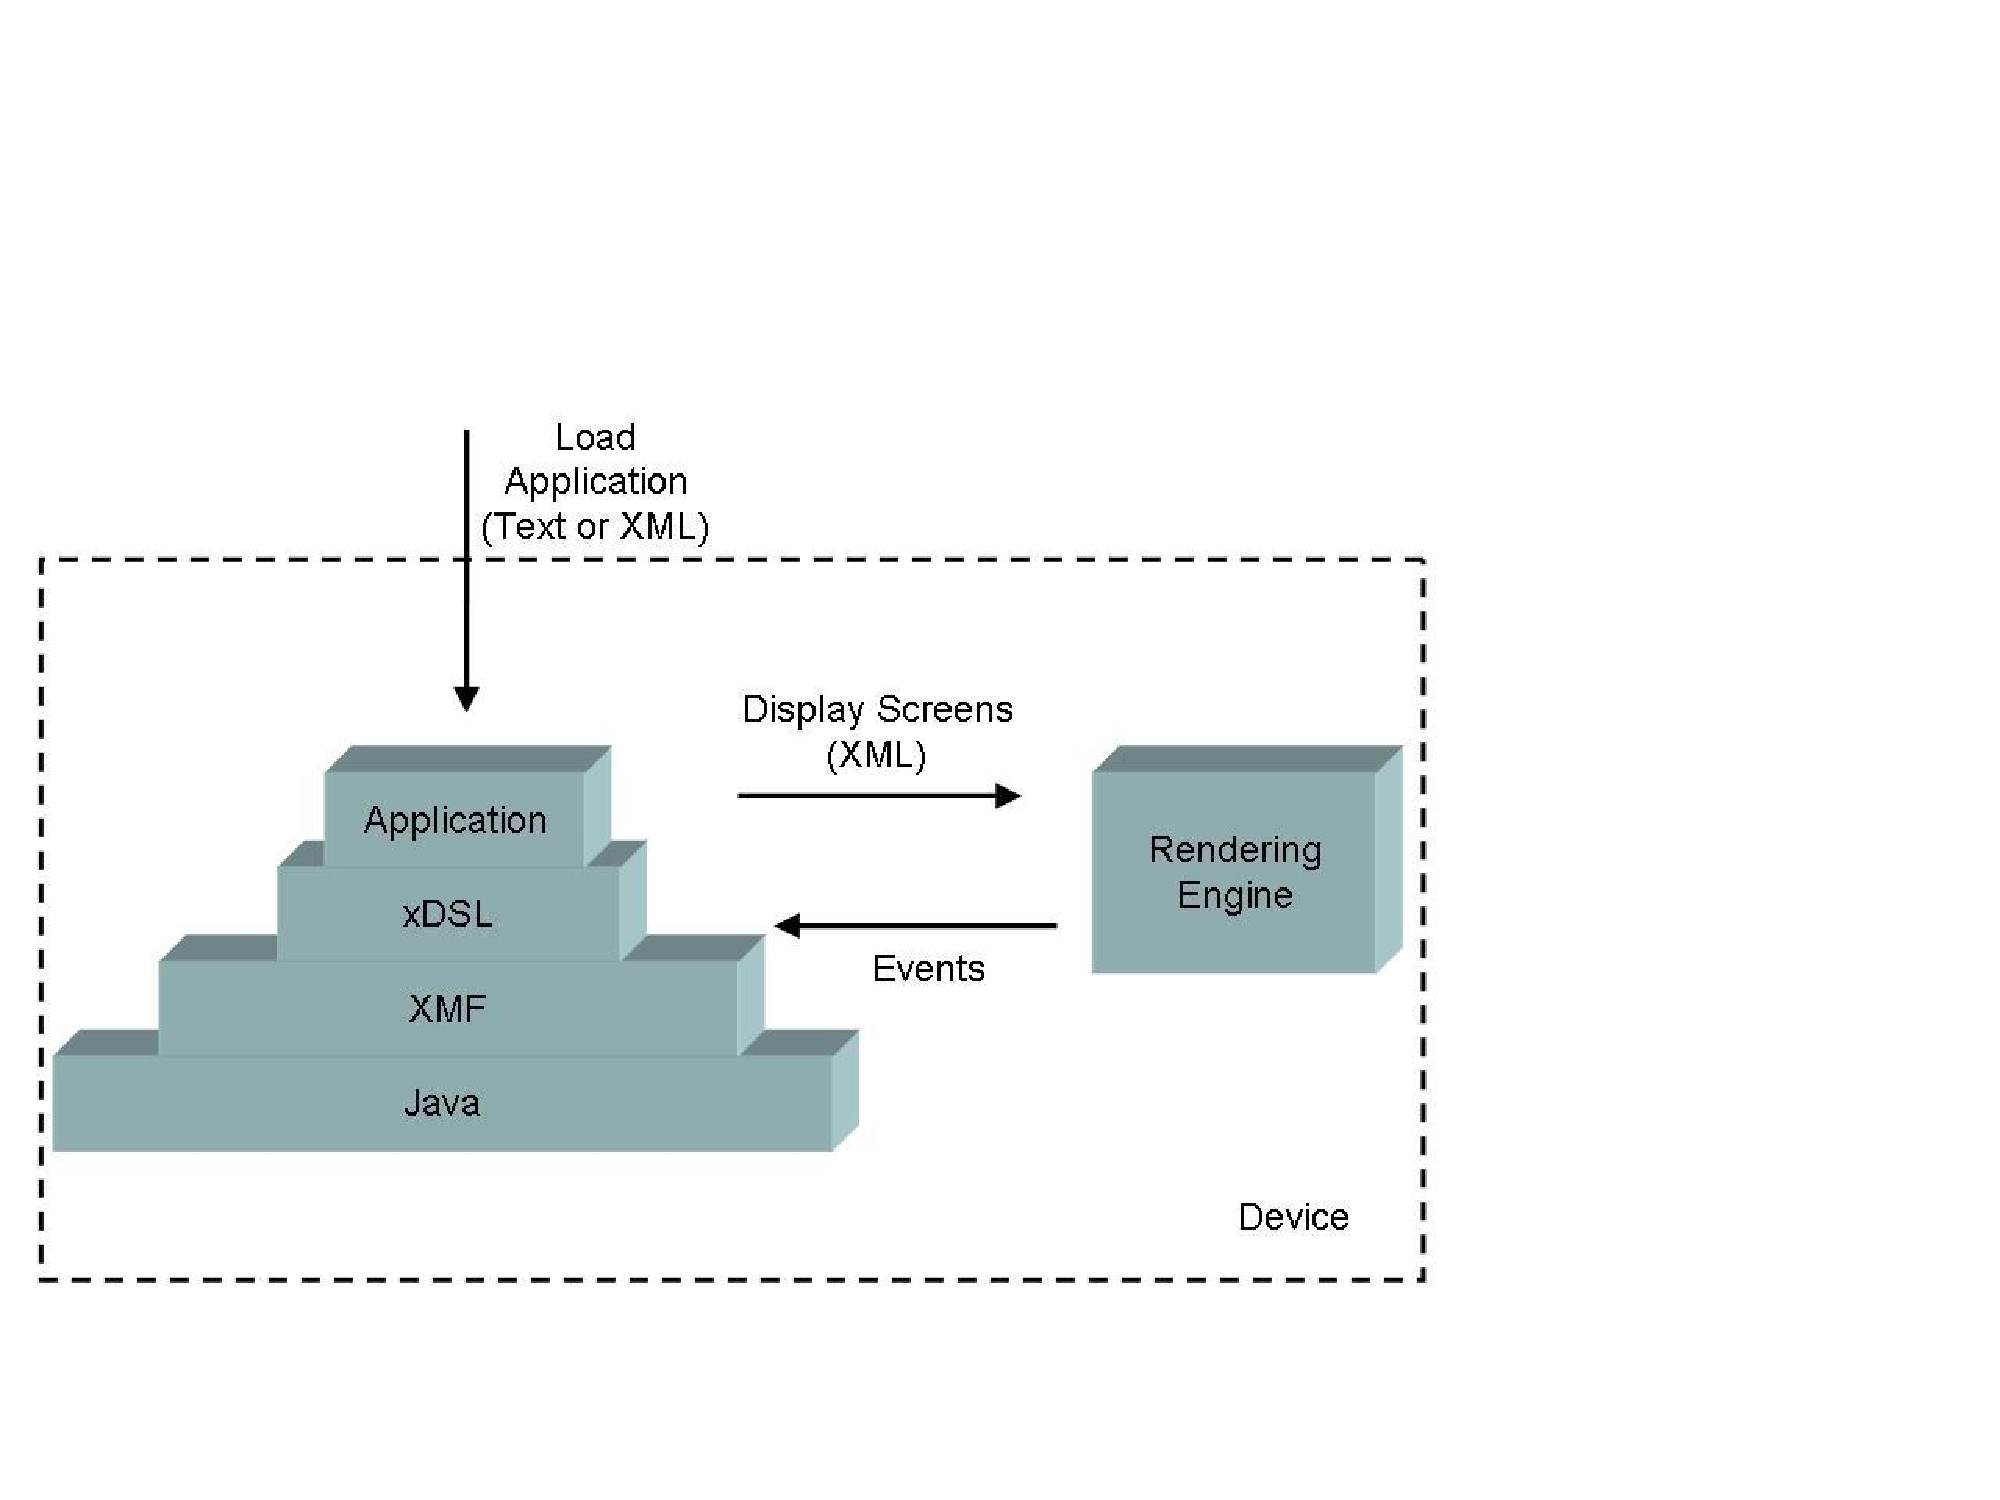
\includegraphics[scale=0.5]{CaseStudy4/figures/Architecture.pdf}

\caption{Application Architecture\label{fig:Application-Architecture}}
\end{center}
\end{figure}


Figure \ref{fig:Application-Architecture} shows an overview of the
architecture for an interactive application xDSL. XMF is used as the
DSL implementation engine. XMF provides facilities for developing
text-based modelling languages and their associated execution engines.
The xDSL is written as a model in XMF, the applications are then loaded
onto the xDSL engine and executed.

The application generates display information in a general-purpose
format; in this case XML. The XML display information is sent to a
rendering engine. The engine understands the display features of the
DSL and interprets them in terms of the rendering technology. This
achieves a separation of concerns whereby the DSL can focus on the
information content and execution logic whereas the rendering engine
can focus on a standard way of displaying the information without
necessarily having to understand anything about the application that
is being rendered.

The rendering engine controls the hardware that interacts with the
user. The user generates events that are sent back to the xDSL engine.
In principle the events can be very detailed and can be encoded in
a suitable DSL. The example presented in this chapter uses a very simple
encoding of events.

When the xDSL receives an event, it must process the data in an appropriate
way to produce more display information for the rendering engine.
The processing information is expressed in the application model running
on the xDSL engine. The display/event loop continues until the application
is terminated.

The architecture shown in figure \ref{fig:Application-Architecture}
has been used a number of times based on the XMF processing engine.
The development environment XMF-Mosaic is completely based upon a
number of rendering engines based on various features of Eclipse:
browsers, property editors and diagram editors. The architecture has
also been successfully used where XMF is deployed as a web-application
and the rendering engine is a standard web-browser (using various
combinations of HTML and the Google Web Toolkit).


\section{A DSL for Interactive Applications\label{sec:A-DSL-for-Interactive-Applications}}

This section presents a simple interactive application expressed using
the xDSL and then shows it running. The following section shows how
the xDSL is implemented in XMF.

Textual languages are developed in XMF by extending the basic language
with new language features. XMF has a small basic language; the rest
is developed by extension. Each new language feature starts with an
'@' character; the feature may be used wherever any normal language
construct is expected. In this way, the XMF engine can be developed
into any special purpose DSL engine.

\newpage{}

The following fragment shows the start of an interactive application:

\begin{lstlisting}
@Model Quiz
  // The Quiz model describes an interactive application
  // for a TV quiz. Viewers are presented with a sequence
  // of questions and get a final score...
  score : Integer;
  // Screen definitions...
end
\end{lstlisting}Each model consists of a collection of screens. Each screen describes
how it is to be rendered and how it responds to events. For example,
the following screen starts the application. It places some text above
a button named Start. When the engine receives a Start event then
the application makes a transition to the screen named Question1:

\begin{lstlisting}
screen START()
  vertical
    text Welcome to the Quiz. Click the button to Start end
    button Start
      go Question1()
    end
  end
end
\end{lstlisting}Options are offered using a construct that lists the options (how
they are displayed is up to the rendering engine). The option group
is named; the name is used to refer to the particular option value
that the user selects when the event returns to the xDSL engine. This
is a typical way of encoding variable information during dialogs:
http does this and can be used to determine the values of fields and
choices on HTML screens. The first part of the Question1 screen uses
options as shown below:

\begin{lstlisting}
screen Question1()
  vertical
    text What is the capital of England? end
    options Choice
      option London; 
      option Paris;
      option Madrid;
    end
    // Question1 continues...
\end{lstlisting}Layout can be handled using many sophisticated schemes. A useful,
simple way to specify layout is to use horizontal and vertical flow,
where these can be nested. The options are displayed below the text
in the fragment given above. In the fragment below, the buttons for
Next and Quit are displayed next to each other (but below the options):

\begin{lstlisting}
    // ... Question1 continues...
    horizontal
      button Next
        // Next action continues...
      end
      button Quit
       go Quit()
      end
    end
  end
end
\end{lstlisting}The Next event is received after the user has chosen an option. If
the option is correct then the user is congratulated and the score
is incremented, otherwise the user is told the correct answer. In
both cases the dialog continues with the next question. 

Actions may be conditional, the conditional expression may refer to
choice variables, values of variables passed to screens and the current
state of the model instance. Actions may also produce displays (without
having to go to a new screen) which allows variables to be scoped
locally within an action %
\footnote{We really should have a let-construct and some local variables here
to show that the nested display has access to locally-scoped variables
over a user-transaction.%
}. In the following, the Next action has two local displays that are
used to respond to the choice:

\begin{lstlisting}
        // ...Next action continues...
        if Choice = "London" 
        then 
          display
            text Well Done end
            button Next
              score := score + 1;
              go Question2()
            end
          end
        else
          display
            text Wrong! Answer is London. end
            button Next
              go Question2()
          end
        end
      end
\end{lstlisting}The DSL is simple and closely matches the concepts required to define
an interactive application. It could be extended in a variety of ways,
for example pattern matching event data and further display concepts.
It includes execution by encoding event handlers. It deals with complexity
by being simple and supporting nesting with local scope and modularity.
A non-expert in interactive software applications should have no problems
writing an application in this DSL.

The following shows a partial execution of this application. Since
there is no rendering engine attached, the XML is printed and the
responses encoded by hand:

\begin{lstlisting}
<Screen>
  <Vertical>
    <Text text=' Welcome to the Quiz. Click the button to Start '/>
    <Button name='Start'/>
  </Vertical>
</Screen>
Start                <-- Event from rendering engine
<Screen>
  <Vertical>
    <Text text=' What is the capital of England? '/>
    <Options name='Choice'>
      <Option name='London'/>
      <Option name='Paris'/>
      <Option name='Madrid'/>
    </Options>
    <Horizontal>
      <Button name='Next'/>
      <Button name='Quit'/>
    </Horizontal>
  </Vertical>
</Screen>
Next Choice=London   <-- Event from rendering engine
<Screen>
  <Text text=' Well Done '/>
  <Button name='Next'/>
</Screen>
Next                 <-- Event from rendering engine
\end{lstlisting}
\section{Implementation\label{sec:Implementation}}

The implementation of the xDSL has two main components: a syntax model
and a grammar that transforms text to instances of the syntax model,
and a semantics model that defines an execution engine. The syntax
model defines a modeling language that defines an application \emph{type};
an instance of the type is defined by the semantics model. This is
a typical way to define a language: models represent things that can
be \emph{performed} in some sense. Performing the models produces
instances whose behaviour is expressed by the model. Another way to
think about this is that we aim to produce libraries of reusable interactive
applications (instances of the syntax model). A run-time occurrence
of an application is described by the semantic model.

XMF provides facilities for working with text including grammars,
XML parsers and XML formatters. The models have been developed using
the XMF development engine XMF-Mosaic and then run on the basic engine.


\subsection{Syntax}

The syntax for the DSL has two parts: the abstract syntax and the
concrete syntax. The abstract syntax consists of a collection of models
that are described below. The concrete syntax is defined by a collection
of grammars that are defined at the end of this section.

%
\begin{figure}
\begin{center}
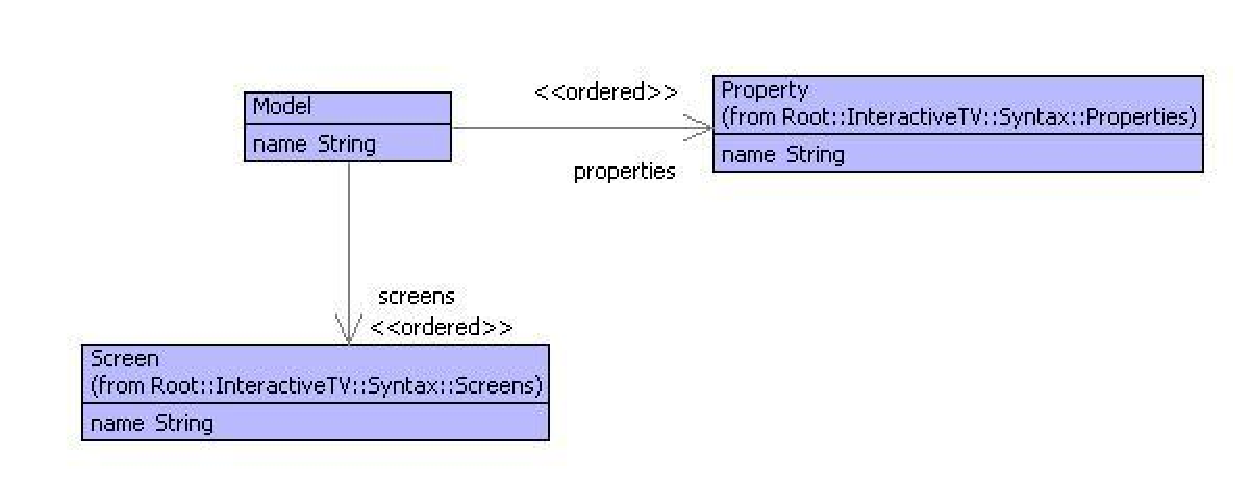
\includegraphics[scale=0.6]{CaseStudy4/figures/Models.pdf}

\caption{Interactive Models\label{fig:Interactive-Models}}

\end{center}
\end{figure}


%
\begin{figure}
\begin{center}
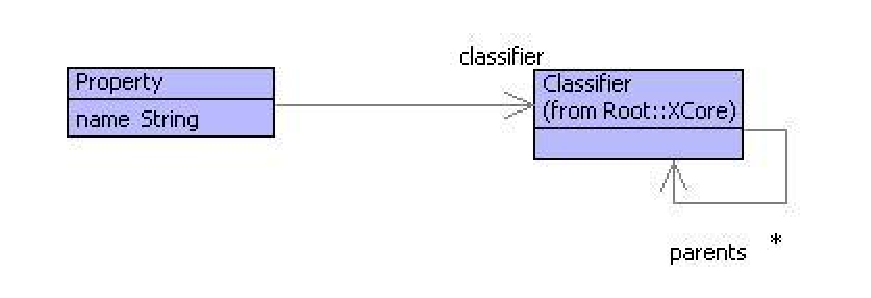
\includegraphics[scale=0.75]{CaseStudy4/figures/Properties.pdf}

\caption{Properties\label{fig:Properties}}

\end{center}
\end{figure}


Figure \ref{fig:Interactive-Models} shows the top-level model for
the interactive application language. A model consists of a collection
of properties and a collection of screens. Each property is defined
by the model in figure \ref{fig:Properties}; it has a name and a
classifier. XMF has a meta-model that provides features such as Class
and Object. A type is called a Classifier in XMF; Integer, String,
Set(Object) are all XMF classifiers.

%
\begin{figure}
\begin{center}
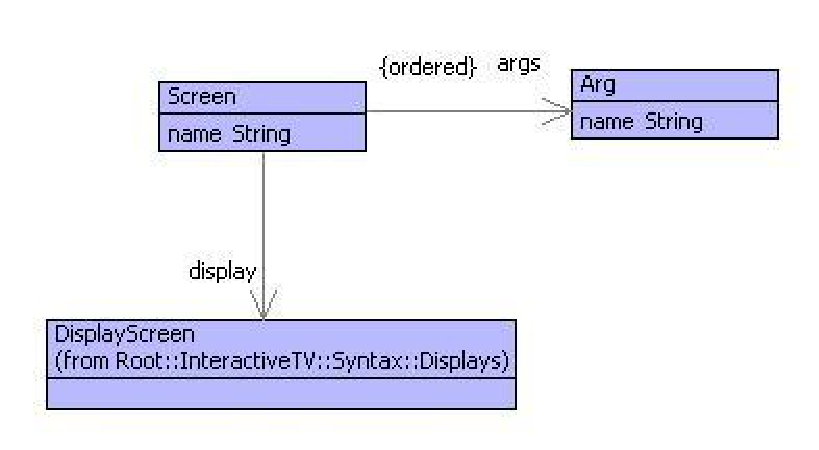
\includegraphics[scale=0.75]{CaseStudy4/figures/Screen.pdf}

\caption{Screens\label{fig:Screens}}
\end{center}
\end{figure}


%
\begin{figure}
\begin{center}
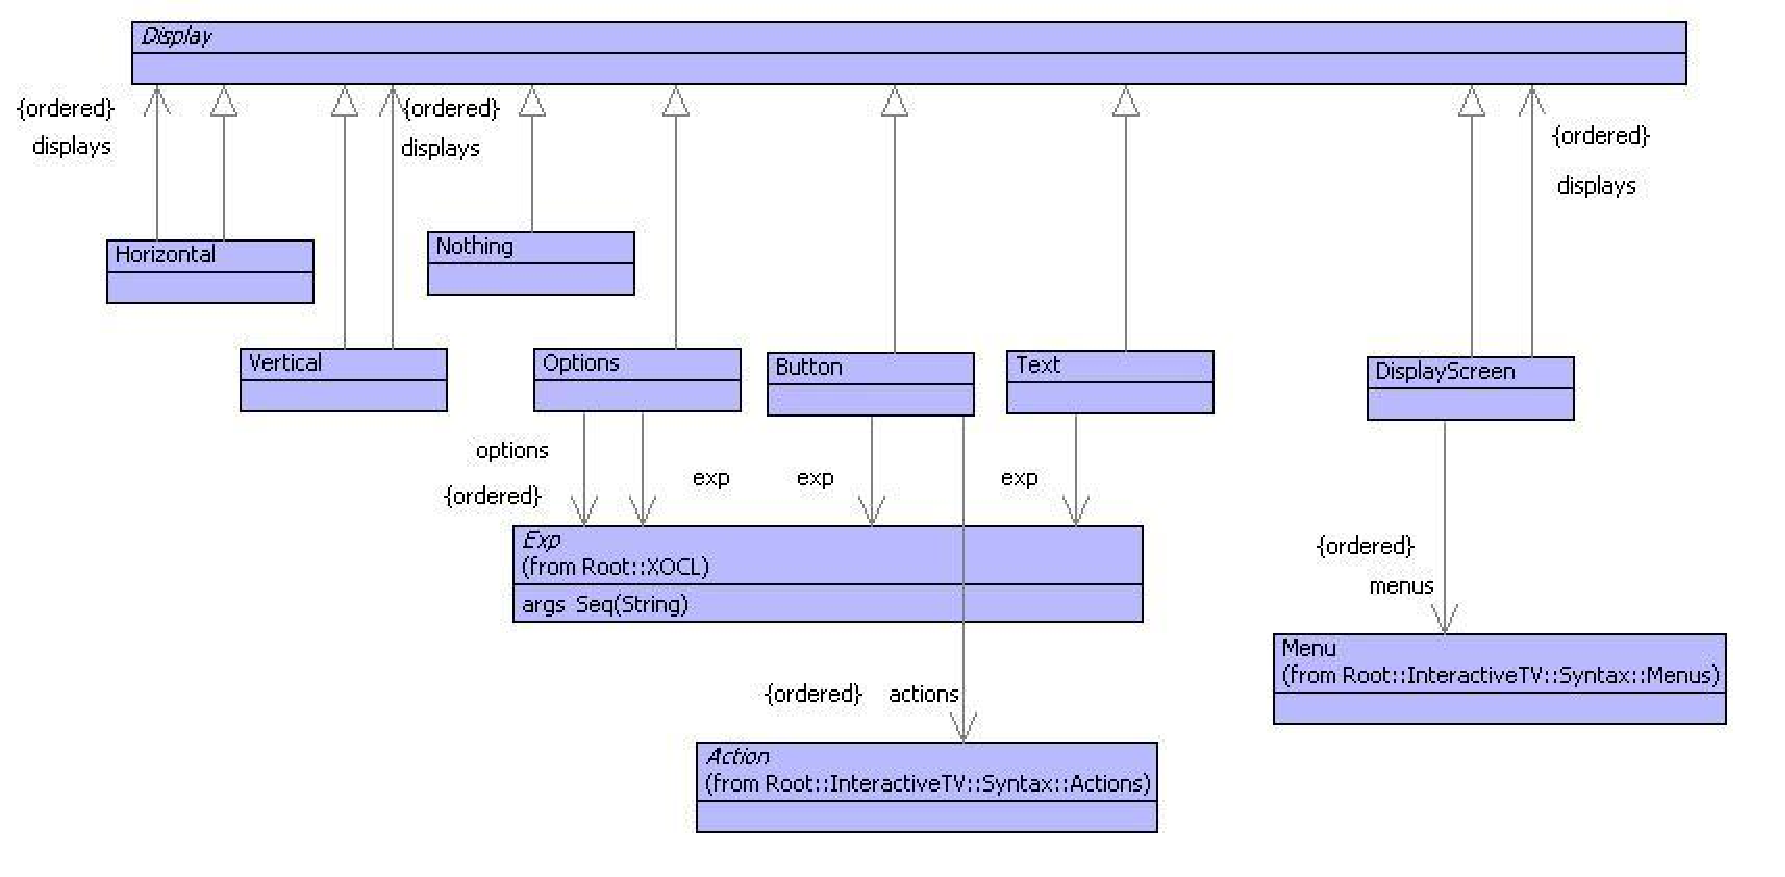
\includegraphics[scale=0.4]{CaseStudy4/figures/Displays.pdf}

\caption{Displays\label{fig:Displays}}
\end{center}
\end{figure}


Screens are shown in figure \ref{fig:Screens}. A screen has a collection
of arguments. An action may cause the application to make a transition
to a screen in which case the transition can supply argument values
to be used when calculating the display for the screen. Figure \ref{fig:Displays}
shows the model for displays. Each element of the display model can
produce XML output that is understood by the rendering engine. In
addition, some of the display elements are associated with actions
that will be performed when the appropriate event is received by the
xDSL engine.

The display elements of an application model refer to an XOCL class
called Exp. This is used wherever an executable fragment of code is
required. It allows features of the displays to be computed dynamically.
For example when a transition to a screen is made, the names of the
buttons may depend on the values of the arguments that are passed
to the screen. This is the reason why a button has an exp: it is used
to calculate the label on the button in terms of the variables that
are in scope at the time%
\footnote{Unfortunately no examples of this feature are given in the document.
However, imagine a list of voting options that will depend on the
current state of the system.%
}. The Exp class is a way of importing the models for XMF expressions
into the displays model.

%
\begin{figure}
\begin{center}
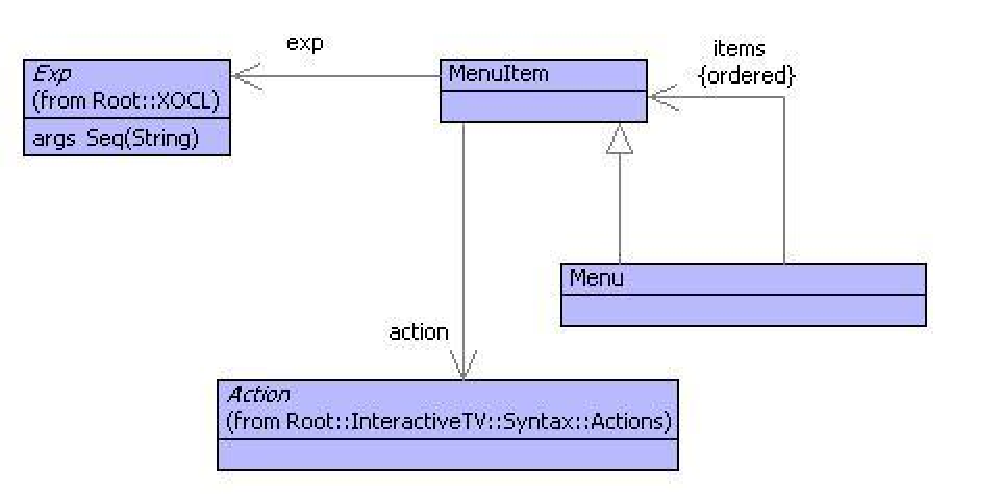
\includegraphics[scale=0.75]{CaseStudy4/figures/Menus.pdf}

\caption{Menus\label{fig:Menus}}
\end{center}
\end{figure}


%
\begin{figure}[htb]
\begin{center}
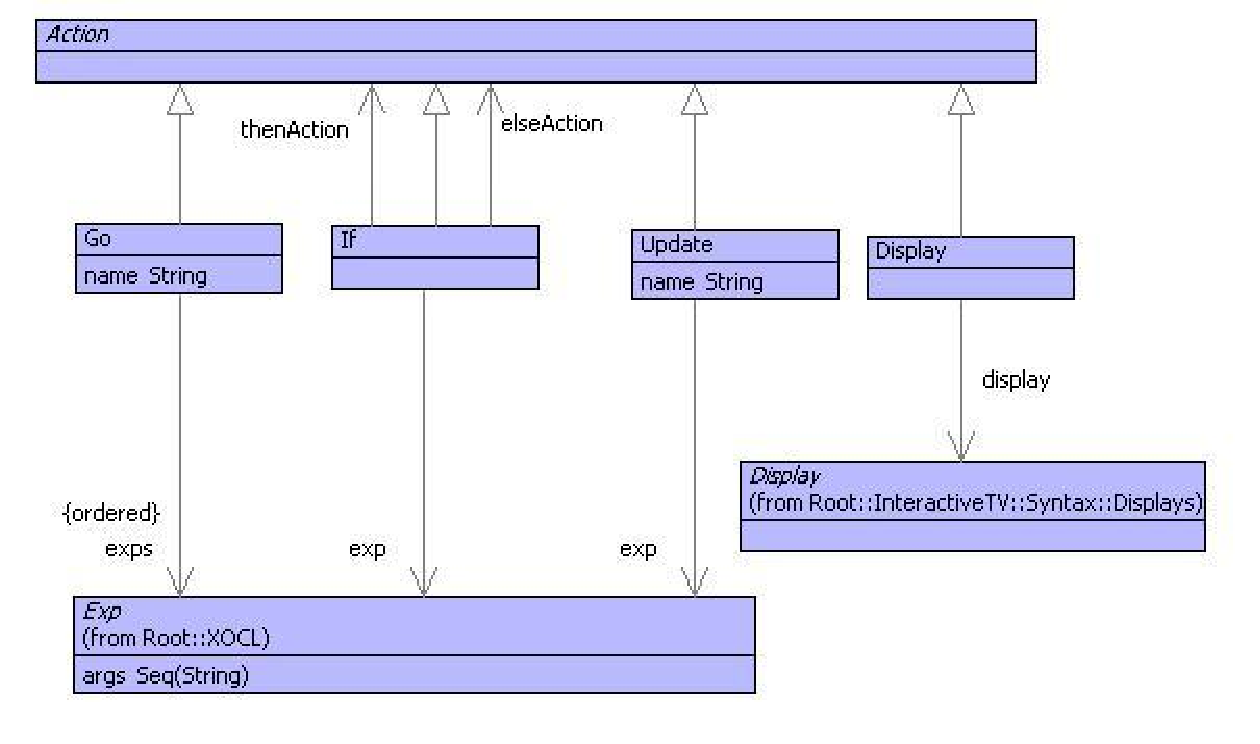
\includegraphics[scale=0.75]{CaseStudy4/figures/Actions.pdf}

\caption{Actions\label{fig:Actions}}
\end{center}
\end{figure}


Menus are shown in figure \ref{fig:Menus}. Each menu has a label
that is computed (again depending on the context) and an action. Actions
are defined in figure \ref{fig:Actions}. An action is either a transition
to a new screen (Go), a conditional action (If), an update to a variable
currently in scope (Update) or a local display.

The developer of an interactive application does not directly create
instances of the abstract syntax model. The idea is that they write
in a text language that is parsed to synthesize instances of the syntax
model%
\footnote{Another way of doing this is to use some form of graphical notation.
XMF is designed to interface to EMF \cite{emf}and GMF \cite{gmf}and
therefore provide execution engines for EMF models. %
}.

XMF allows any class to be extended with a grammar. The class then
defines a new syntax construct that is completely integrated into
the base language of XMF. Any number of classes can be added in this
way and new syntax classes can build on existing syntax classes. The
following is a simple example of a class definition that implements
a simple guarded expression:

\begin{lstlisting}
@NotNull [e1].m(e2,e3,e4)
  else e5
end
\end{lstlisting}where e1 evaluates to produce an object to which we want to send the
message m with args e2,e3 and e4. However, e1 might produce null in
which case we don't want to send the message, we want to do e5 instead.
This language construct is implemented as follows in XMF:

\newpage{}

\begin{lstlisting}
@Class NotNull extends Sugar

  @Attribute exp       : String            end
  @Attribute name      : String            end
  @Attribute isMessage : Boolean           end
  @Attribute args      : Seq(Performable)  end
  @Attribute error     : Performable       end
    
  @Constructor(exp,name,error) end
    
  @Constructor(exp,name,args,error) 
    self.isMessage := true
  end
    
  @Grammar extends OCL.grammar
    NotNull ::= 
      '[' e = Exp ']' '.' n = Name NotNullTail^(e,n) 'end'.
      
    NotNullTail(e,n) ::= 
      '(' as = NotNullArgs ')' x = NotNullElse { NotNull(e,n,as,x) }
    | x = NotNullElse { NotNull(e,n,x) }.
      
    NotNullArgs ::=
      e = Exp es = (',' Exp)* { Seq{e|es} }
    | { Seq{} }.
      
    NotNullElse ::=
      'else' Exp 
    | { [| null |] }.
      
  end
    
  @Operation desugar():Performable
    [| let notNullValue = <exp>
       in if notNullValue = null
          then <error>
          else <if isMessage
                then Send([| notNullValue |],name,args)
                else [| notNullValue.<name> |]
                end>
          end
       end
    |]
  end
    
end
\end{lstlisting}The key features of the NotNull class are as follows:

\begin{itemize}
\item The class extends Sugar which means that it is defining a new syntax
construct by providing an operation called 'desugar' whose responsibility
is to turn an instance of NotNull into program code.
\item The grammar definition extends the OCL grammar and thereby imports
all of the basic grammar-rule definitions. This provides the rule
for Exp which is the top-level grammar-rule for all language constructs.
\item Each grammar-rule consists of a name and a body. The rule may optionally
have arguments. The body consists of terminals (in ' and'), builtins
such as Name, rule-calls (possibly with arguments) and actions (inside
\{ and \}). The rule actions are any program expression, in most cases
they use class-constructors to create an instance of a named class.
\item The desugar operation uses lifting-quotes ({[}| and |]) to create
an instance of syntax-classes. The opposite of \emph{lifting} is \emph{dropping}
(< and >) used to calculate syntax by evaluating a program expression.
\end{itemize}
The rest of this section describes how the grammar feature of XMF
can be used to define the interaction language. A model consists of
a name followed by properties and screen definitions:

\begin{lstlisting}
context Model
  @Grammar extends Property.grammar, Screen.grammar
     Model ::= n = Name ps = Property* ss = Screen* 'end' {
        Model(n,ps,ss)
      }.
  end
\end{lstlisting}A property is a name and a simple expression (that cannot include
the ';' operator). The property-rule action uses an interesting feature
of syntax classes that allows the expression to be dropped into the
syntax element and is thereby evaluated to produce a classifier for
the property type:

\begin{lstlisting}
context Property extends OCL::OCL.grammar
  @Grammar extends OCL.grammar
    Property ::= n = Name ':' e = SimpleExp ';' {
      Property(n,Drop(e))
    }.
  end
\end{lstlisting}A screen has a name, arguments, menus and display elements. The rule
for screen arguments shows how optional elements are processed: it
returns either a non-empty sequence of names Seq\{a|as\} (head followed
by tail) or the empty sequence Seq\{\}:

\begin{lstlisting}
context Screen
  @Grammar extends Menu.grammar, Display.grammar
    Screen ::= 
      'screen' n = Name '(' as = ScreenArgs ')' 
         ms = Menu* 
         ds = Display* 
      'end' { Screen(n,as,DisplayScreen(ms,ds)) }.
    ScreenArgs ::=
      a = Name as = (',' Name)* { Seq{a|as} }
    | { Seq{} }.
  end
\end{lstlisting}A menu is shown below. This shows how expressions are captured in
data. The rule for a menu item name returns an instance of the class
Exp that is used in data to wrap an evaluable expression. There are
two forms of construction for Exp: Exp(e) and Exp(e,V,null). In both
cases e is an instance of a syntax class. In the second case V is
a collection of variable names that occur freely in e. The values
of variables in V can be supplied when the expression is evaluated
(via keyApply as shown below).

Another interesting feature of the menu item name rule is the use
of 'lift' to transform a data element (in this case a string n) into
an expression whose evaluation produces the original data element:

\begin{lstlisting}
context Menu
  @Grammar extends OCL.grammar
    Menu ::= 'menu' n = MenuItemName is = MenuItem* 'end' {
      Menu(n,is)
    }.
    MenuItemName ::= 
      n = Name { Exp(n.lift()) }
    | e = SimpleExp { Exp(e,e.FV(),null) }.
    MenuItem ::=
      Menu
    | 'item' n = MenuItemName a = Action 'end' { MenuItem(n,a) }.
  end
\end{lstlisting}\newpage{}

Since Display is an abstract class, the grammar-rule for Display is
a list of concrete alternatives:

\begin{lstlisting}
context Display
  @Grammar extends Action.grammar, OCL.grammar
    Display ::=
        Text
      | Button
      | Options
      | Horizontal
      | Vertical.
    Text ::= 'text' t = Char* 'end' { 
      Text(Exp(t.asString().lift())) 
    }.
    Button ::= 
      'button' n = ComputedName 
        as = Action* 
      'end' { Button(n,as) }.
    ComputedName ::=
      n = Name { Exp(n.lift()) }
    | e = SimpleExp { Exp(e,e.FV(),null) }.
    Options ::= 
      'options' n = ComputedName 
        os = Option* 
      'end' { Options(n,os) }.
    Option ::=
      'option' n = Name ';' { n }.
    Horizontal ::=
      'horizontal'
        ds = Display*
      'end' { Horizontal(ds) }.
    Vertical ::=
      'vertical'
        ds = Display*
      'end' { Vertical(ds) }.
  end
\end{lstlisting}\newpage{}

Action is another example of an abstract class:

\begin{lstlisting}
contxt Action
  @Grammar extends OCL.grammar
    Action ::=
        UpdateProperty
      | IfAction
      | Go
      | DisplayScreen.
      DisplayScreen ::= 
        'display' 
          ms = Menu* 
          ds = Display* 
        'end' { DisplayScreen(ms,ds) }.
      UpdateProperty ::=
        n = Name ':=' e = SimpleExp ';' {
          Update(n,Exp(e,e.FV(),null))  
      }.
      Go ::= 'go' n = Name '(' as = GoArgs ')' { Go(n,as) }.
      GoArgs ::= 
        e = GoArg es = (',' GoArg)* { Seq{e|es} }
      | { Seq{} }.
      GoArg ::= e = SimpleExp { Exp(e) }.
      IfAction ::=
        'if' e = SimpleExp
        'then' d = Action
        IfActionTail^(e,d).
      IfActionTail(e,d1) ::=
        'else' d2 = Action 'end' { If(Exp(e,e.FV(),null),d1,d2) }
      | 'end' { If(Exp(e,e.FV(),null),d1,null) }. 
  end
\end{lstlisting}
\subsection{Semantics}

%
\begin{figure}
\begin{center}
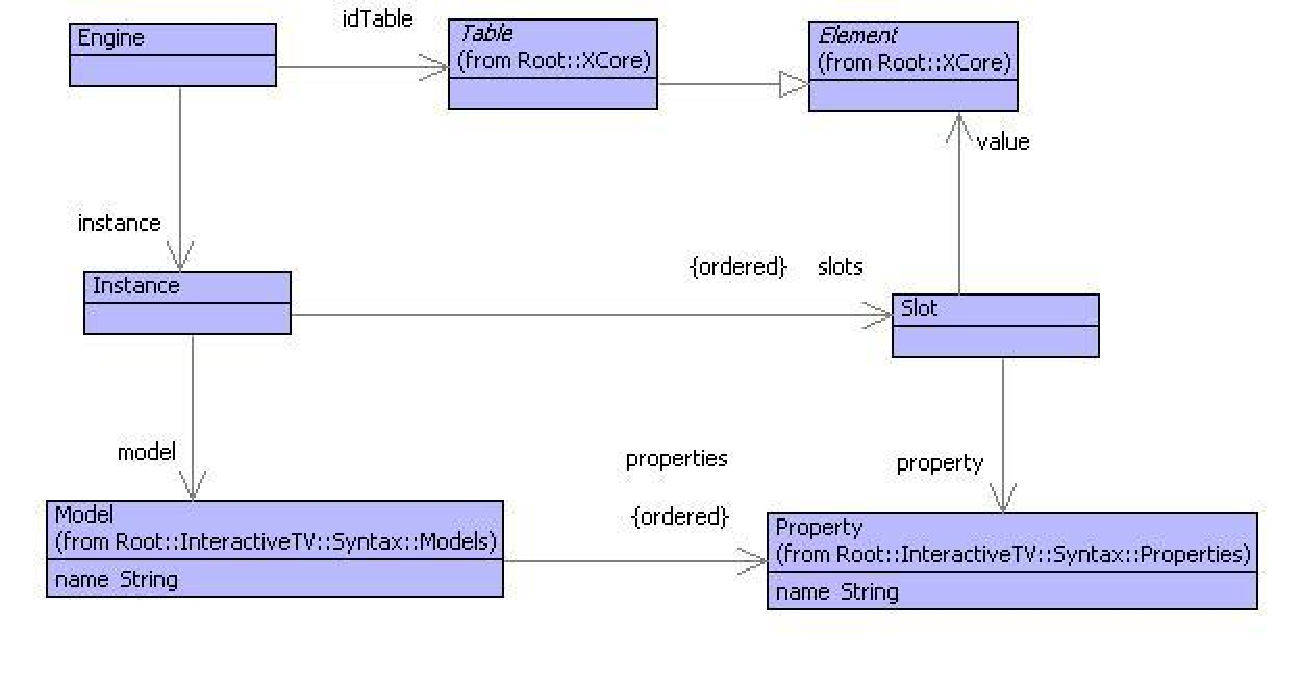
\includegraphics[scale=0.6]{CaseStudy4/figures/Engine.pdf}

\caption{Semantics Model\label{fig:Semantics-Model}}
\end{center}
\end{figure}


The semantics of the interactive application modelling language defines
an instance model for the syntax and also defines an execution engine
for the instances. The instance model is shown in figure \ref{fig:Semantics-Model}.
An instance of a Model is defined by the class Instance. It should
have a slot for each property of the model. The value of each slot
should have a type that is defined by the classifier of the corresponding
property.

The class Engine defines the execution engine. An engine controls
an instance and maintains an id-table that maps event ids to handlers
as shown below. The idea is that each time an event occurs, a handler
from the id-table is used to produce a new XML display that is sent
to the rendering engine. The XML data is calculated from the information
in the model and the current state of the instance slots.

The rest of this section defines the engine execution semantics. The
following section shows how the engine is connected to a rendering
engine. The engine processes a screen-transition using the 'go' operation
defined below. XMF supports many types of input and output channel.
The 'go' operation shows an example of a string output channel used
to capture and then return the XML output data as a string:

\begin{lstlisting}
context Engine
  @Operation go(screen:String,args:Seq(Element))
    let sout = StringOutputChannel()
    in instance.go(screen,args,self,sout);
       sout.getString()
    end
  end
\end{lstlisting}An instance handles a screen-transition by looking up the screen in
its model. If the screen exists then it is requested to display itself
with the supplied argument values:

\begin{lstlisting}
context Instance
  @Operation go(screen:String,args:Seq(Element),engine:Engine,out:OutputChannel)
    @NotNull [model.indexScreensByName(screen,null)].display(self,args,engine,out)
      else self.error("No screen called " + screen)
    end
  end
\end{lstlisting}A screen delegates the 'display' message to its underlying display
component. The screen argument names are bound to the argument values
to produce an \emph{environment of bindings} using the 'env' operation:

\begin{lstlisting}
context Screen
  @Operation display(instance,args,engine,out)
    display.display(instance,self.env(instance,args),engine,out)
  end
context Screen    
  @Operation env(instance,values)
    let env = args.zip(values)
    in instance.slots()->iterate(slot env = env | 
         env.bind(slot.property().name(),slot.value()))
    end
  end
\end{lstlisting}Each display element type : Button; Text; Horizontal; Vertical; and,
Options implements a 'display' operation that writes XML data to the
supplied output channel. As a side effect, if any of the elements
have event handling actions then the engine is updated with an appropriate
handler for the event when it is received from the rendering engine.

Each 'display' operation shows the use of an XMF language feature
@XML ... end that is used to write XML output to a channel. The construct
has the form:

\begin{lstlisting}
@XML(out)
  <TAG ATTS>
    .. program code ...
  </TAG>
end
\end{lstlisting}where the literal XML data is written to the supplied output channel.
In-between writing the starting tag and ending tag, an arbitrary program
is processed.

\begin{lstlisting}
context DisplayScreen
  @Operation display(instance,env,engine,out)
    @XML(out)
      <Screen>
        @For menu in menus do
          menu.display(instance,env,engine,out)
        end
        @For display in displays do
          display.display(instance,env,engine,out)
        end
      </Screen>
    end
  end
\end{lstlisting}The 'display' operation for text shows an example of the shortened
form of the XML construct with no body, and also the use of the 'keyApply'
operation of the Exp class. The 'env' argument supplied to 'display'
contains bindings for all variables in scope. The 'keyApply' operation
performs the expression in the context of these variables:

\begin{lstlisting}
context Text
  @Operation display(instance,env,engine,out)
    @XML(out)
      <"Text" text=exp.keyApply(env)/>
    end
  end
\end{lstlisting}A button contains an action that is used to handle the event arising
from the user pressing the button in the rendering engine. The 'display'
operation for Button shows how an event handler is registered in the
engine. The arguments passed to 'registerActions' are the context
required to perform the actions when the event associated with 'id'
is received:

\begin{lstlisting}
context Button
  @Operation display(instance,env,engine,out)
    let id = exp.keyApply(env)
    in engine.registerActions(id,instance,env,actions);
       @XML(out)
         <Button name=id/>
       end
    end
  end
\end{lstlisting}Horizontal and Vertical are similar:

\begin{lstlisting}
context Horizontal
  @Operation display(instance,env,engine,out)
    @XML(out)
      <Horizontal>
        @For display in displays do
          display.display(instance,env,engine,out)
        end
      </Horizontal>
    end
  end
\end{lstlisting}\newpage{}

The 'display' operation for Options shows an example of interleaving
of XML and program code:

\begin{lstlisting}
context Options
  @Operation display(instance,env,engine,out)
    @XML(out)
      <Options name=exp.keyApply(env)>
        @For option in options do
          @XML(out)
            <Option name=option/>
          end
        end
      </Options>
    end
  end
\end{lstlisting}The 'registerActions' operation of Engine must define a handler for
an event. The definition associates the event identifier 'id' with
an operation in the id-table of the engine. Actions are performed
using their 'perform' operation which expects to receive arguments
that include the current environment of variable bindings. The variables
available to an action include all those bound by selecting options
on the display. These display-bound variables are supplied to the
handler (in the same way that http works) as an environment 'env2':

\begin{lstlisting}
contxt Engine
  @Operation registerActions(id,instance,env1,actions)
    idTable.put(id,
      @Operation(env2)
        let value = null
        in @For action in actions do
             value := action.perform(instance,env2 + env1,self)
           end;
           value
        end
      end)
  end
\end{lstlisting}There are four types of action: If; Update; Go; and, Display. Each
action produces a result and the last action performed should return
an XML string to be sent to the rendering engine. If performs one
of two actions (or nothing) depending on the outcome of a test:

\begin{lstlisting}
context If
  @Operation perform(instance,env,engine)
    if exp.keyApply(env + instance.env())
    then thenAction.perform(instance,env,engine)
    else @NotNull [elseAction].perform(instance,env,engine) end
    end
  end
\end{lstlisting}An update changes the value of a variable currently in scope. The
variables in scope are: the slots of the instance; the current screen
arguments. The following operation checks whether the named variable
is a slot and updates the instance appropriately, or updates the current
environment:

\begin{lstlisting}
context Update
  @Operation perform(instance,env,engine)
    @NotNull [instance.getSlot(name)].setValue(exp.keyApply(env + instance.env()))
      else env.set(name,exp.keyApply(env + instance.env()))
    end
  end
\end{lstlisting}Go makes a transition to a new screen. The screen will produce the
XML output. Notice that the current 'env' is not supplied to the 'go'
operation; therefore any variables currently in scope are not available
to the target screen unless their values are passed as arguments:

\begin{lstlisting}
context Go
  @Operation perform(instance,env,engine)
    engine.go(name,exps->collect(exp | exp.keyApply(env)))
  end
\end{lstlisting}Display is a way of locally displaying a screen without losing the
variables that are currently in scope:

\begin{lstlisting}
context Display
  @Operation perform(instance,env,engine)
    let sout = StringOutputChannel()
    in display.perform(instance,env,engine,sout);
       sout.getString()
    end
  end
\end{lstlisting}
\subsection{Handling Events}

Events occur when the user interacts with the rendering engine, for
example by pressing a button. When the event occurs, the current screen
may contain any number of option groups. Each option group is named
and offers a number of alternative values. The selected option may
affect the behaviour of the engine in terms of variable updates and
screen transitions. Therefore, the event sent from the rendering engine
to the xDSL engine must encode the value of any option variables currently
displayed.

In addition there may be any number of ways an event can be raised:
menu selection or button press. Each must be uniquely identified and
the event must supply the identifier of the event that occurred. 

An event is defined to have a format that starts with the event id
and is followed by any number of option variable/value pairs:

\begin{lstlisting}
<ID> <VAR>=<VALUE> ... <VAR>=<VALUE>
\end{lstlisting}The event is encoded as a string and must be decoded by the engine.
This is easily done by defining an event as a grammar-rule:

\begin{lstlisting}
context Engine
  @Grammar
    Event ::= n = Name e = Binding* { Seq{n|e} }.
    Binding ::= n = Name '=' v = Name { Seq{n|v} }.
  end
\end{lstlisting}When an event is received by the engine it is supplied to 'getDisplay'
which calculates a new XML display string for the rendering engine.
The operation uses the grammar defined above to synthesize a pair
Seq\{id|env\} containing the event id and an environment of option-group
variable bindings. If the id is bound in the id-table then the handler
is supplied with the environment:

\begin{lstlisting}
context Engine
  @Operation getDisplay(event:String)
    let pair = Engine.grammar.parseString(event,"Event",Seq{}) then
        id = pair->head;
        env = pair->tail
    in @TableGet handler = idTable[id] do
         idTable.clear();
         handler(env)
       else self.error("No handler for " + name)
       end
    end
  end
\end{lstlisting}
\section{Simulation\label{sec:Simulation}}

Figure \ref{fig:Application-Architecture} shows the architecture
of an interactive application. The rendering engine is external to
the design of an xDSL; the relationship between the two is defined
by the XML schema for the display language and the format of event
strings. However, it is useful to be able to simulate the rendering
engine in order to test the xDSL engine. This can be done by setting
up a simple test harness for a pair of data consumers and linking
the xDSL engine with a rendering engine simulation that reads events
strings in from the terminal.

\newpage{}

The following class implements a data producer-consumer pair:

\begin{lstlisting}
@Class Consumer

  @Attribute filter : Operation end
  @Attribute other  : Consumer (!) end
    
  @Constructor(filter) ! end
    
  @Operation consume(data)
    other.consume(filter(data))
  end
end
\end{lstlisting}The filter operation is used to generate data that is supplied to
the other consumer. If a pair of Consumer instances are linked together
then the data will bounce back and forth as required. The following
operation creates a filter for the xDSL engine:

\begin{lstlisting}
@Operation mk_xDSL_filter(model:Model)
  let engine = Engine(model.new())
  in @Operation(event)
       engine.getDisplay(event)
     end
  end
end
\end{lstlisting}The following filter operation simulates the rendering engine. It
does so by pretty-printing the XML to the standard-output. An XML
string can be transformed into an XML tree using the 'asXML' operation
defined for String. The standard-input is flushed and a line containing
the event is read and returned:

\begin{lstlisting}
@Operation renderFilter(xml:String)
  xml.asXML().pprint(stdout);
  "".println();
  stdin.skipWhiteSpace();
  stdin.readLine().stripTrailingWhiteSpace()
end 
\end{lstlisting}Given a model 'model', the following code produces, and starts, a
simulation:

\begin{lstlisting}
@Operation simulate(model:Model)
  let eConsumer = Consumer(mk_xDSL_filter(model));
      dConsumer = Consumer(renderFilter)
  in eConsumer.setOther(dConsumer);
     dConsumer.setOther(eConsumer);
     eConsumer.consume("START")
  end
end
\end{lstlisting}
\section{XML Representation for Applications\label{sec:XML-Representation-for}}

A requirement for interactive applications is to be able to dynamically
update the content and to be able to transfer the content from remote
locations in a standard format. The application describes in this
chapter is completely represented in data. This means that, although
the application is executable, it can easily be serialized, sent over
a communications link, and then uploaded onto the device that is running
the xDSL engine.

XMF provides support for encoding any data elements as XML. There
is a basic markup provided for all XMF data; the mechanisms for which
can easily be extended to provide bespoke XML encoding. Using the
basic mechanisms, a model can be encoded as follows:

\begin{lstlisting}
@WithOpenFile(fout -> "c:/model.xml")
  let xout = XMLOutputChannel(fout,NameSpaceXMLFormatter())
  in xout.writeValue(model)
  end
end
\end{lstlisting}%
\begin{figure}
\begin{center}
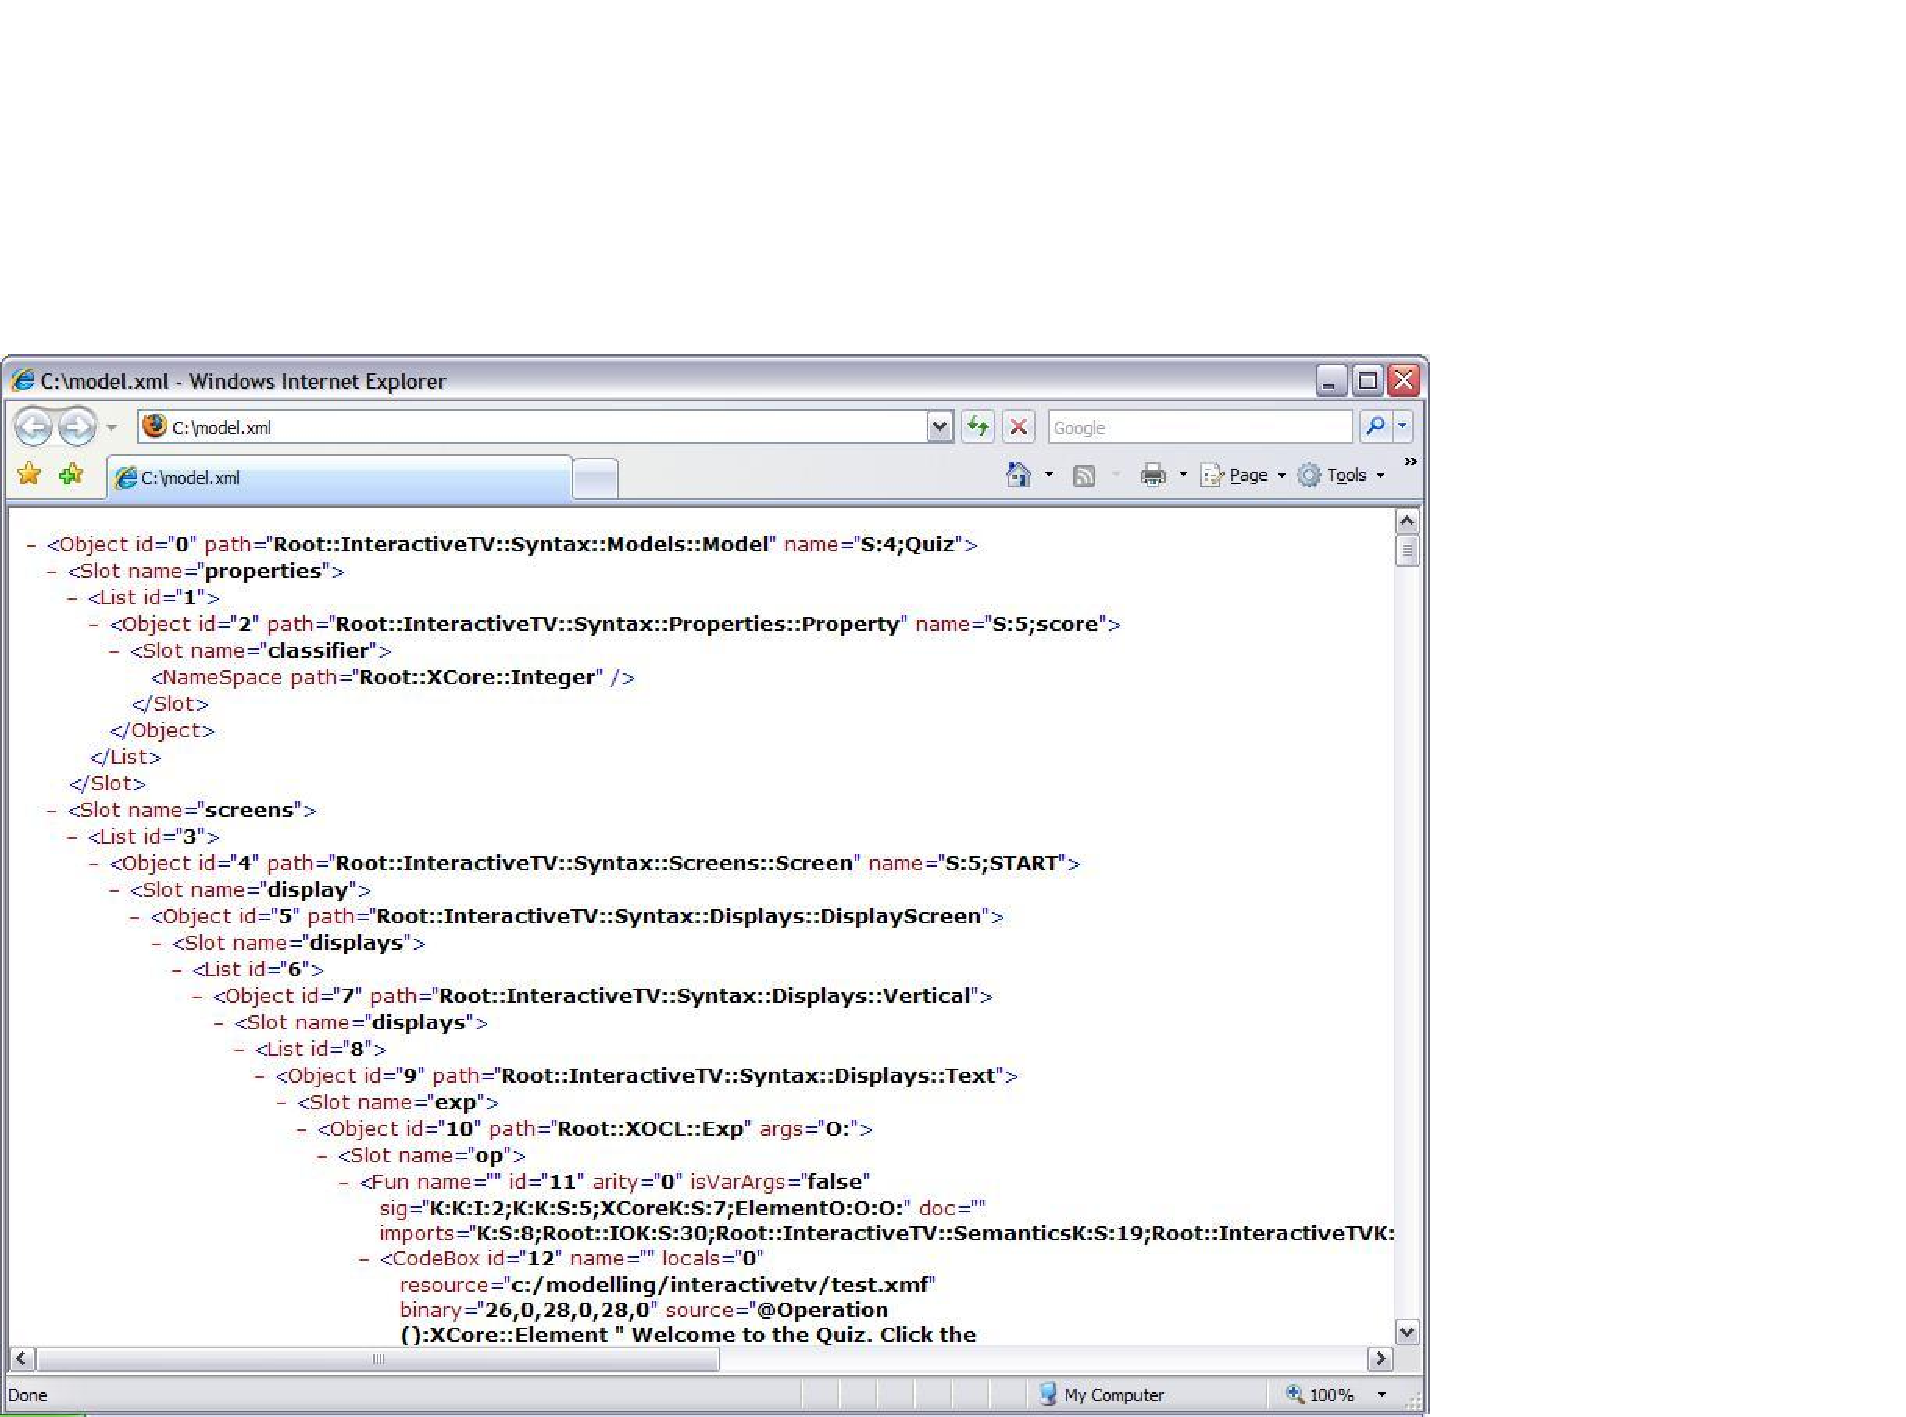
\includegraphics[scale=0.6]{CaseStudy4/figures/Serialized.pdf}

\caption{A Serialized Model\label{fig:A-Serialized-Model}}
\end{center}
\end{figure}

The resulting output is produced in an XML file that is shown in figure
\ref{fig:A-Serialized-Model}. The XML markup shown in the figure
is the default vanilla-flavour markup provided by XMF. It is possible
to add adapters to an XML output channel that filter the data as it
is processed and thereby use domain-specific markup. So instead of
seeing Object and Slot as element tags, we might use Screen and Button.

The XML can be read back in using the following code:

\begin{lstlisting}
@WithOpenFile(fin <- ModelFile)
  let xin = XMLInputChannel(fin,NameSpaceXMLInflater())
  in xin.parse()
  end
end
\end{lstlisting}
\section{Conclusion\label{sec:Conclusion}}

This chapter has described an approach to modelling systems whereby
an engine for an executable domain-specific language (xDSL) is used
to develop and run the applications. The xDSL is designed to use concepts
that are suited to the application domain which allows the language
to abstract away from implementation details; the language is then
executable, can be used with different implementation platform technologies,
and is suitable for use by people whose primary skill lies in the
application domain rather than the implementation technology.

A method for developing xDSLs has been shown that involves a separation
of concerns between syntax elements that describe type-level features
of a model, and semantics elements that define run-time features of
an application. Experience has shown that this separation is natural
and allows the xDSL developer to effectively manage the process.

We have shown how a textual syntax can be added to an xDSL. In practice,
most xDSLs will require a concrete syntax. The precise form of this
will depend on the nature of the application and who the intended
users are. Sometimes, a purely graphical syntax is appropriate (for
example UML class-diagrams). Other times a purely textual syntax works
best, especially where executable features are involved and when complexity
can be controlled effectively using textual nesting. Often there is
scope for a mixture of the two where different aspects of the models
are constructed using graphical or textual syntax.

Modelling all features of a language has a number of benefits that
arise because everything is \emph{reified}. Reification involves representing
everything as data as opposed to program code or transient non-tangible
artifacts such as system events. Once everything is reified, many
types of analysis are possible including well-formedness checking,
type checking, application of style rules. It becomes easy to capture
and apply patterns and to perform refactoring. All features of an
application can be transformed to a target technology. 

Modelling actions is particularly important here; often actions are
left as unprocessed strings of program code which makes it very difficult
to analyze and run as part of an xDSL engine. The application given
in this paper has shown that it is straightforward to model actions
and to integrate them into the execution engine for an xDSL. By following
a few basic guidelines in terms of variable scope and control flow,
actions are easy to implement and are completely integrated into the
xDSL, its analysis and transformation.

The approach models the xDSL and executes it directly using an engine
(in this case XMF). This is attractive because it provides a high
degree of control over the language. It should be contrasted with
a translational approach to implementing a DSL whereby the model is
translated to the source code of a target language (such as Java or
C++) for which there is an implementation platform. This is an approach
taken by Swul \cite{SWUL} and GMF \cite{gmf} for GUI applications.
Translational approaches have some advantages: notably open architectures;
efficiency; arbitrary extensibility. However, there are some significant
disadvantages relating to the complexity of the generated code including
maintainability and understandability. It should be noted that an
xDSL engine-based approach does not preclude a translational approach.

We have given a complete implementation of an interactive application
xDSL using the features of XMF. XMF is an engine that is specifically
designed to support this kind of application development. It has very
high-level language features that support modelling concepts, it is
executable, and is designed to support textual language extension
through the use of extensible grammars. XMF directly supports textual
xDSLs and provides native interfaces to Java and EMF/GMF for use with
other concrete syntaxes.

XMF may be used to develop an xDSL and then deploy the language as
a stand-alone engine as shown in figure \ref{fig:Application-Architecture}.
XMF runs its own virtual machine and has a number of interface features
that allow it to connect to external applications. XMF may also be
used to develop an executable design of an application which is then
exported on to another implementation platform.